% ===== CHAPTER 5: TESTING =====

\chapter{Testing}
\label{ch:testing}

At mid-semester the project had one widget test, and Section~\ref{sec:analysis} called
that the biggest hole in the work. This chapter records how it was closed. Testing ran at
four levels: unit and widget tests inside the Flutter app, end-to-end tests that drive the
real server and database through its public API, system testing of the finished app on an
iPhone simulator, and static analysis.

\section{Test Plan and Environment}

\begin{table}[H]
\centering
\begin{tabular}{|L{3.2cm}|L{8.3cm}|}
\hline
\textbf{Level} & \textbf{What it covers and how it runs} \\
\hline
Unit and widget (app) & 19 tests in \texttt{frontend/test}, run with
\texttt{flutter test}. They check the host form's inputs, the activity/event chooser,
the category list, the notification banner, date formatting, the saved login and the
navigation stack after login. \\
\hline
End-to-end (server) & 29 tests in \texttt{backend/test/api.test.js}, run with
\texttt{npm test} using Node's built-in test runner. Each test signs up its own users
through the real API, so every check passes through routing, the JWT middleware, the
controllers, MySQL transactions and, for TC23, the Socket.IO server. \\
\hline
System (manual) & The app built for an iPhone 17 Pro simulator and pointed at the test
server, walked through every user-facing case with fictional seeded students.
Screenshots are in Section~\ref{sec:screens}. \\
\hline
Static analysis & \texttt{flutter analyze} with the \texttt{flutter\_lints} rules. \\
\hline
\end{tabular}
\caption{Levels of testing}
\label{tab:testlevels}
\end{table}

\noindent\textbf{Environment.} A MacBook Air (Apple M3, 8~GB) running macOS~27, Node.js
24.4, MySQL 9.7 and Flutter 3.47, with the iOS 26.5 simulator.

\medskip
\noindent\textbf{Keeping test data away from real data.} The server tests create accounts,
send one-time codes and ban users, so they never touch the development database. They run
against a separate database, \texttt{campus\_companion\_test}, built from
\texttt{schema.sql}, and the suite refuses to start unless the database name contains
``test''. The server under test sends mail to a small SMTP sink on the same machine that
accepts and discards everything, and is given dummy Twilio credentials, so no e-mail or text
message reaches a real person. Codes are read from the \texttt{otp\_verifications} table
instead of an inbox. The suite was run three times in a row against the same database
without a failure, so it does not depend on starting from an empty one.

\section{Server Test Cases}

Table~\ref{tab:apitests} lists every server test case with the result of the final run on
20 November 2026. ``Expected'' is what the test asserts, not a paraphrase of it.

\begin{longtable}{|p{1.0cm}|L{4.2cm}|L{4.4cm}|p{1.4cm}|}
\caption{End-to-end server test cases and results}\label{tab:apitests}\\
\hline
\textbf{ID} & \textbf{Scenario} & \textbf{Expected} & \textbf{Result} \\
\hline
\endfirsthead
\hline
\textbf{ID} & \textbf{Scenario} & \textbf{Expected} & \textbf{Result} \\
\hline
\endhead
\hline
\endfoot
TC01 & Register with a \texttt{@gmail.com} address & 400, message names \texttt{@thapar.edu} & Pass \\ \hline
TC02 & Register without a gender & 400, ``Gender is required'' & Pass \\ \hline
TC03 & Log in before entering the code & 403 with \texttt{requiresVerification} & Pass \\ \hline
TC04 & Enter a wrong code, then the right one & 400 ``Incorrect'', then 200 & Pass \\ \hline
TC05 & Enter a code after it has expired & 400 ``expired'' & Pass \\ \hline
TC06 & Ask for a new code within 60 s & 429 & Pass \\ \hline
TC07 & Register an already verified address & 409 & Pass \\ \hline
TC08 & Wrong password vs.\ unknown address & Both 401 with the same message & Pass \\ \hline
TC09 & Forgot password, known vs.\ unknown address; reset with a short then a valid password & Same 200 message for both; 400 for short; old password then refused, new one accepted & Pass \\ \hline
TC10 & Use a sign-up code to reset a password & 400 & Pass \\ \hline
TC11 & Call a protected route with no token or a forged one & 401 both times & Pass \\ \hline
TC12 & Host with category ``More\ldots'' or ``Event'' & 400 both times & Pass \\ \hline
TC13 & Host an activity & Host is a participant and a member of its chat & Pass \\ \hline
TC14 & Host asks to join their own activity & 400 & Pass \\ \hline
TC15 & A third student lists or accepts requests & 403; the host's accept returns 200 & Pass \\ \hline
TC16 & Host accepts a request & Guest is added to the group chat & Pass \\ \hline
TC17 & Declined student asks again & 403 & Pass \\ \hline
TC18 & Ask to join a full activity & 409 & Pass \\ \hline
TC19 & Two accepts sent at the same instant for the last place & One 200 and one 409; exactly two participants & Pass \\ \hline
TC20 & Rate before the end; after it, rate self, rate 4.3, rate as an outsider, then a valid 4.5 with one real and one made-up tag & 400; 400; 400; 403; 200 with only the real tag stored & Pass \\ \hline
TC21 & View another student's public profile & 200, no e-mail, phone or emergency contact in the response & Pass \\ \hline
TC22 & Event with a Football activity in teams of 2; outsider signs up; accepted guest joins directly; guest starts a team & Refused; 400 (must join a team); team created & Pass \\ \hline
TC23 & Host sends a chat message; an outsider tries to join the room and send & Member receives it live; outsider refused both times & Pass \\ \hline
TC24 & SOS with no emergency contact saved & 400, message asks for a contact & Pass \\ \hline
TC25 & Ordinary user calls an admin route & 403 & Pass \\ \hline
TC26 & Admin bans a user who is already logged in & Old token 403, login 403 with the reason, socket refused; admin cannot ban self & Pass \\ \hline
TC27 & Upload a 6~MB avatar, then a text file & 400 JSON both times & Pass \\ \hline
TC28 & ID check with one photo, then with two blank photos & 400; then 422 \texttt{NOT\_THAPAR\_CARD}, status \texttt{failed} & Pass \\ \hline
TC29 & ID check from a non-student address & 422 \texttt{EMAIL\_FORMAT} & Pass \\ \hline
\end{longtable}

\noindent The one positive ID card case, a real card verifying its owner, is not in the
automated suite because it needs photographs of a real student's card, which do not belong
in a repository. It was tested by hand on 19 November against both sides of a real card:
the owner passed from two different front photos, and another student's e-mail, swapped
photos, a second front photo instead of the back, and a non-student e-mail were each refused
with their own message.

\section{App Test Cases}

\begin{table}[H]
\centering
\begin{tabular}{|L{3.3cm}|p{1.1cm}|L{5.6cm}|p{1.4cm}|}
\hline
\textbf{File} & \textbf{Tests} & \textbf{What is checked} & \textbf{Result} \\
\hline
\texttt{\footnotesize categories} & 4 & Every category the host form can post has a Discover chip; no duplicates; the ``All'' chip comes first and is not itself postable & Pass \\
\hline
\texttt{\footnotesize host\_choice} & 4 & The Host button offers activity or event; each opens the right form; the event form has no category picker; Event is never offered for an ordinary activity & Pass \\
\hline
\texttt{\footnotesize host\_inputs} & 3 & Number fields accept typed values and clamp them; two side by side at phone width still show their digits; the date and time sheet returns what was picked & Pass \\
\hline
\texttt{\footnotesize when\_format} & 3 & Single-day times, multi-day date ranges, and an event that is still running counts as not ended & Pass \\
\hline
\texttt{\footnotesize notification\_popup} & 2 & A pushed notification slides in and hides; several arrive one at a time & Pass \\
\hline
\texttt{\footnotesize auth\_session} & 1 & A login survives a restart until Log Out & Pass \\
\hline
\texttt{\footnotesize login\_stack} & 1 & After login there is nothing to swipe back to & Pass \\
\hline
\texttt{\footnotesize widget} & 1 & With no saved login the app opens on the login screen & Pass \\
\hline
\end{tabular}
\caption{Flutter unit and widget tests}
\label{tab:fluttertests}
\end{table}

\section{Test Runs}

Figures~\ref{fig:run-api} and~\ref{fig:run-flutter} are the console output of the final
runs, unedited apart from line length. \texttt{flutter analyze} reported ``No issues found''
on the same code.

\begin{figure}[H]
\centering
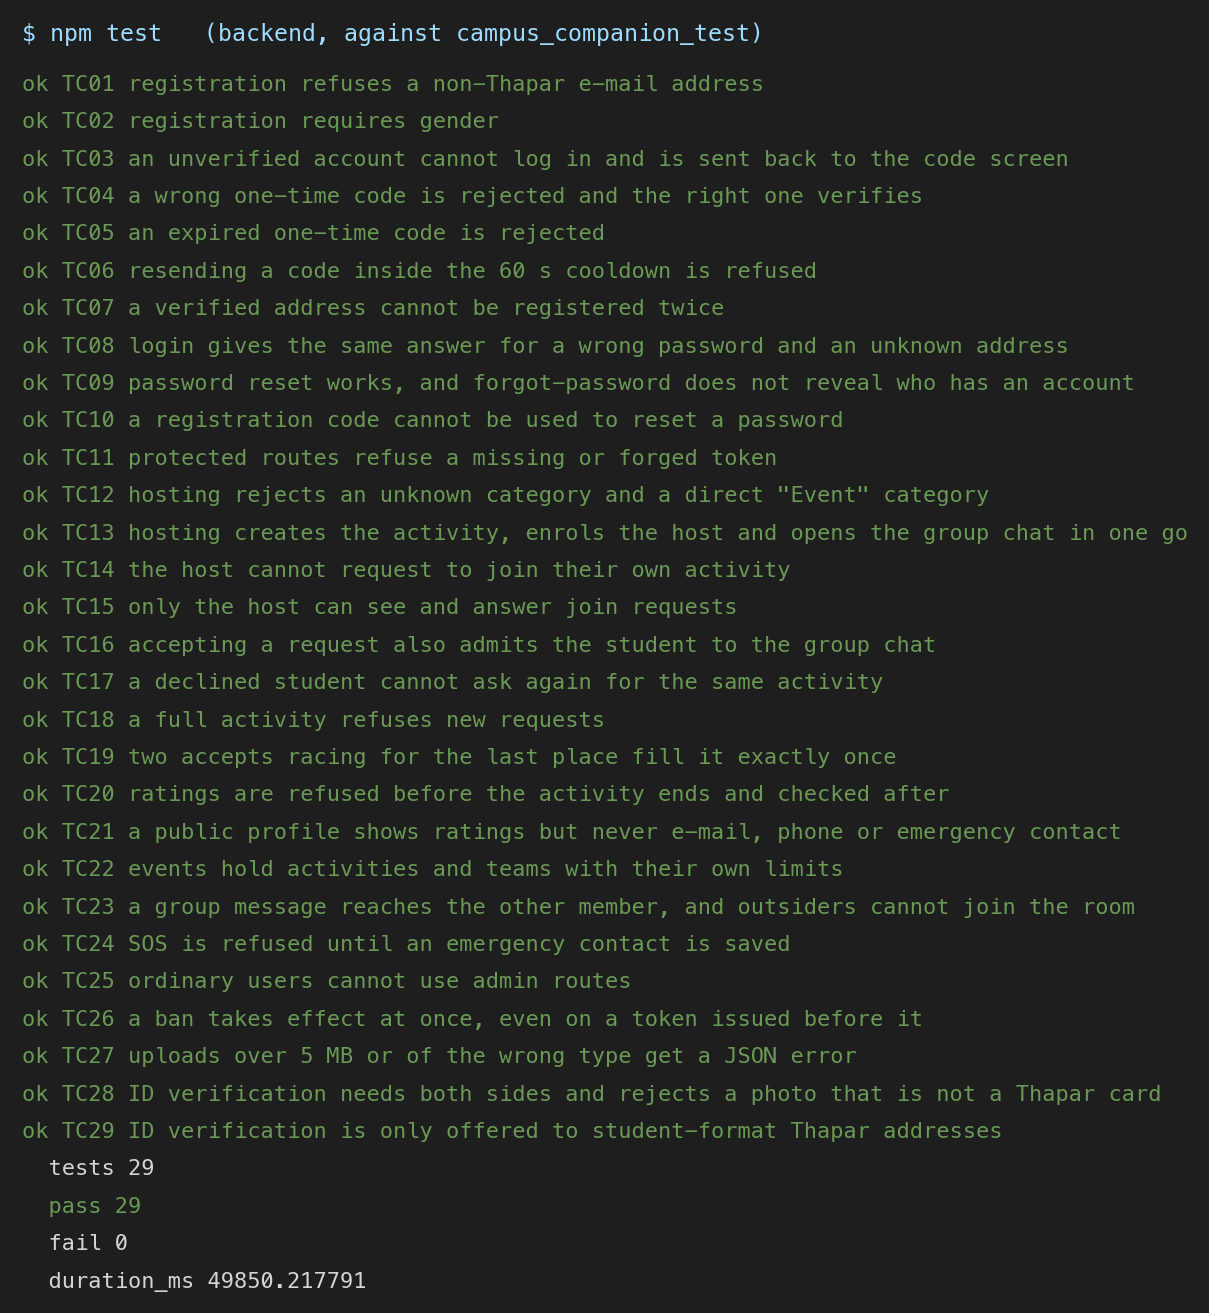
\includegraphics[width=\textwidth]{figures/charts/run-api-tests.png}
\caption{Final run of the server suite: 29 of 29 passing}
\label{fig:run-api}
\end{figure}

\begin{figure}[H]
\centering
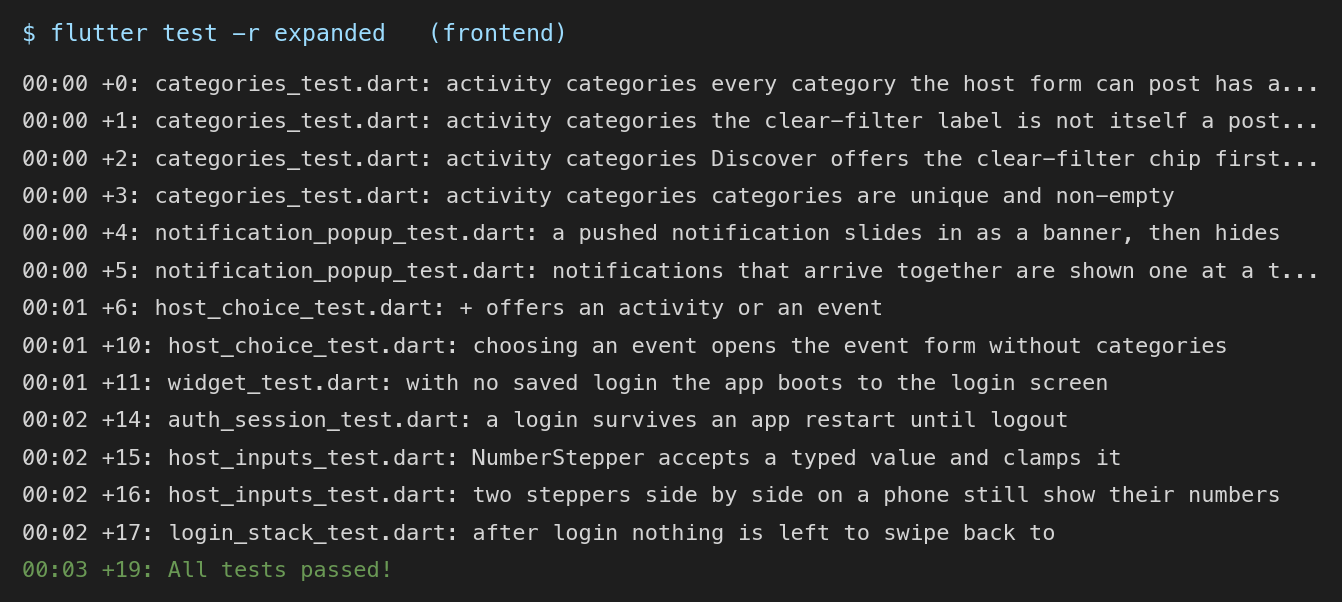
\includegraphics[width=\textwidth]{figures/charts/run-flutter-tests.png}
\caption{Final run of the Flutter suite: 19 of 19 passing}
\label{fig:run-flutter}
\end{figure}

\section{System Testing on the Simulator}
\label{sec:screens}

For system testing the app was built for the iPhone 17 Pro simulator against the test
server, and the database was filled with five fictional students, six activities, one event
with three activities inside it, a finished walk with ratings and reviews, and a short group
chat. Figures~\ref{fig:scr-join} to~\ref{fig:scr-safety} show the screens as they
appeared, each labelled with the test case it supports.

\newcommand{\screen}[2]{%
  \begin{minipage}[t]{0.29\textwidth}\centering
    \includegraphics[width=\linewidth]{figures/screens/#1}\\[2pt]
    {\footnotesize #2}
  \end{minipage}}

\begin{figure}[p]
\centering
\screen{01-login.png}{(a) Login; only \texttt{@thapar.edu} accepted (TC01, TC08)}\hfill
\screen{04-discover.png}{(b) Discover with the featured event pinned and category chips (TC12)}\hfill
\screen{14-host-choice.png}{(c) Host asks: activity or event}\\[10pt]
\screen{15-host-form.png}{(d) Host form with the five categories (TC12, TC13)}\hfill
\screen{05-activity-host.png}{(e) Host's view with two pending requests (TC15)}\hfill
\screen{06-accepted.png}{(f) After accepting Dev: 3/4 people, Dev under Who's In (TC16)}
\caption{Signing in, browsing, hosting and the join handshake}
\label{fig:scr-join}
\end{figure}

\begin{figure}[p]
\centering
\screen{07-group-chat.png}{(a) Group chat opened from the activity page (TC23)}\hfill
\screen{08-event.png}{(b) Event with Football in teams of five and the Red Hawks team (TC22)}\hfill
\screen{10-notifications.png}{(c) Notifications for acceptance, reviews and requests}\\[10pt]
\screen{09-profile.png}{(d) Own profile: 4.5 from 3 ratings, histogram and tags (TC20)}\hfill
\screen{16-public-profile.png}{(e) Another student's public profile, with no contact details (TC21)}\hfill
\screen{17-admin-profile.png}{(f) The same profile seen by an admin: Ban and Give red tick (TC25, TC26)}
\caption{Chat, events, notifications, profiles and moderation}
\label{fig:scr-profile}
\end{figure}

\begin{figure}[p]
\centering
\screen{18-verify-id.png}{(a) ID card check for an unverified account (TC28)}\hfill
\screen{11-settings.png}{(b) Settings for a verified student, with the red tick}\hfill
\screen{12-emergency-contact.png}{(c) Emergency contact saved (TC24)}\\[10pt]
\screen{13-sos.png}{(d) Pressing SOS still shows ``SOS isn't set up yet, coming soon''}
\caption{Identity and safety}
\label{fig:scr-safety}
\end{figure}

\clearpage
\section{Defects Found During Final Testing}

Writing and running the tests found the following. Defects found and fixed earlier, while
the features were being built, are recorded in the journal in Chapter~\ref{ch:journal}.

\begin{enumerate}
  \item \textbf{\texttt{schema.sql} failed on a fresh MySQL install.} It used
        \texttt{ADD COLUMN IF NOT EXISTS}, which only MariaDB supports, so creating the
        test database stopped at line 19 with only the \texttt{users} table made. Nobody
        had hit it because the development database predates those lines. Fixed: every
        table now declares all its columns, and \texttt{migrate.js} covers older databases.
  \item \textbf{TC28 passed for the wrong reason.} Its first version used a non-student
        address, so the request was refused on the e-mail format before the card photos
        were ever read. The test passed while checking nothing about the card. It was
        caught because the test took 120~ms, too fast for OCR to have run. Fixed: TC28 now
        uses a student-format address and asserts \texttt{NOT\_THAPAR\_CARD}, and the
        e-mail check got its own case, TC29.
  \item \textbf{TC26 only worked on an empty database.} On a database where the test admin
        account already existed with another password, it failed before reaching the ban.
        Fixed by giving that account the run's password first.
  \item \textbf{The activity search box on Discover does nothing} (Section~\ref{sec:impl}).
        Found while taking the screenshots. Not fixed.
  \item \textbf{The SOS control is still a placeholder} (Figure~\ref{fig:scr-safety}d). Known
        since mid-semester. Not fixed.
\end{enumerate}
